% Practice Exam A: questions and solutions in one source. \input by
% midterm2-practice-a.tex (\solutionsfalse) and
% midterm2-practice-a-solutions.tex (\solutionstrue). Two parts weighted
% equally at 10 points each, each on its own sheet printed front and back, with
% name and CWID boxes on every sheet. Part 2 is a percentage tax on soda, read off a
% graph with no equations (Div, 2026-11-03). This repo is public: keep notes
% about the real exam out of this file. Numbers are checked in
% figures/make_midterm2.py.

% No points on the parts: the grading scheme gets decided later (Div, 2026-11-03).
\renewcommand{\qpart}[2]{\par\vspace{10pt}\noindent(#1) }

\ifsolutions
\docheader{Practice Exam A: Solutions}{ECON 201}
\else
\sheet{Sheet 1 of 2}
\docheader{Practice Exam A}{ECON 201}
\begin{notepanel}{Instructions}
\begin{itemize}
\item 60 minutes. Two parts, weighted equally at 10 points each, each on its own sheet printed front and back: Part 1, ten multiple-choice questions; Part 2, one long-form question.
\item Closed book and closed notes. Bring a basic calculator. There is no help sheet, since there is not much to put on one: the only formulas you might need are for the area of a triangle or a rectangle, and any question that needs one will give it.
\item Write your name and CWID, one digit per box, at the top of every sheet: the sheets are graded separately and matched by CWID.
\item Show your work and explain your answers in Part 2.
\end{itemize}
\end{notepanel}
\fi

\section{Part 1: Multiple Choice \pts{10}}
\where{Fill the bubble of the one best answer.}

\begin{enumerate}\setlength{\itemsep}{4pt}

\mcq{At a price of \$50, 30 students want to buy used skis and 70 want to sell. What do we expect to happen?}
  {The price rises, since there is excess demand of 40.}
  {The price stays at \$50, since some skis still sell.}
  {The price falls, since there is excess supply of 40.}
  {The price rises, since there is excess supply of 40.}
\sol{(C). At \$50, 70 are offered and 30 are wanted, an excess supply of 40. Sellers with unsold skis have an incentive to lower their price.}

\mcq{A shortage pushes up the price of copper. How do buyers and producers respond to the higher price?}
  {Buyers use less or find substitutes, and producers supply more.}
  {Buyers buy more before it rises, and producers hold back their copper.}
  {Buyers change nothing, and producers cut their output.}
  {Buyers use more, and producers supply less.}
\sol{(A). At a higher price, some buyers no longer find copper worth its price, and units that were not worth producing before can now be sold at a profit.}

\mcq{Many stands sell the same roasted corn at a going price of \$3. Why does no stand charge more or less than \$3?}
  {The stands have agreed with each other to charge \$3.}
  {Above \$3 it sells nothing, and at \$3 it can sell all it likes.}
  {Buyers care about the stand but not about the price of corn.}
  {The city has set the price of roasted corn at \$3.}
\sol{(B). With identical goods, buyers go to another stand if one charges more. A stand is small, so it can already sell all it wants at \$3, and charging less would only cut its profit.}

\mcq{A price-taking farm can grow 40 crates of peaches at a marginal cost of \$2 each and 20 more at \$7 each. The going price is \$5. How many crates does it grow?}
  {0}
  {20}
  {60}
  {40}
\sol{(D). A price-taker produces every unit whose marginal cost is below the price. The first 40 add $5 - 2 = 3$ each, and the next 20 would each lose $7 - 5 = 2$.}

\mcq{The farms in a competitive market form a cartel and hold the price above the market-clearing level. What happens?}
  {Total surplus rises, since farms earn more on each unit.}
  {Fewer units are sold, so some trades with WTP above MC are lost.}
  {More units are sold, since farms want to sell more at a higher price.}
  {Total surplus stays the same, since buyers lose what farms gain.}
\sol{(B). At the higher price buyers want less, and trade happens on the short side. Units with WTP above MC go unsold, and that lost surplus is the deadweight loss. Farms may gain, but buyers lose more than farms gain.}

\mcq{Demand for lumber shifts right by the same amount in two markets. Supply is steep in one and flat in the other. What happens?}
  {The price rises more with flat supply, and the quantity rises more there too.}
  {The price rises by the same amount in both, since the shift is the same.}
  {The price rises more with steep supply, and the quantity rises less there.}
  {The price rises more with steep supply, and the quantity rises more there too.}
\sol{(C). With steep supply, extra units cost much more to produce, so the price has to rise a lot to bring them out, and the quantity rises only a little.}

\mcq{A popular show makes more people want pickleball paddles at every price. In this competitive market:}
  {supply shifts right, and quantity demanded rises along the demand curve.}
  {demand shifts right, and supply shifts right.}
  {demand shifts left, and quantity supplied falls along supply.}
  {demand shifts right, and quantity supplied rises along supply.}
\sol{(D). The shock changes what buyers want at every price, so demand shifts. The marginal costs of paddle makers have not changed, so supply stays put and sellers respond to the higher price along their supply curve.}

\mcq{After a rise in demand, sellers keep selling out at the old price. What happens next?}
  {Prices rise, more is supplied, and some buyers drop out, until the market clears.}
  {Prices stay at the old level, since no one knows the new equilibrium price.}
  {Prices fall, since sellers have sold more than they expected to sell.}
  {Prices rise until the quantity sold falls back to its old level.}
\sol{(A). Buyers who go without would pay more, and sellers notice they could charge more. As the price rises, sellers offer more and some buyers decide it is no longer worth it. This goes on until buyers want exactly what sellers offer.}

\mcq{Which of these is a long-run shift in the supply of coffee?}
  {A frost raises the cost of picking this year's crop.}
  {New farms enter after years of high coffee prices.}
  {The coffee price rises, and existing farms pick more.}
  {Cafes buy more coffee at every price.}
\sol{(B). In the long run the number of firms and their capacity can change. (A) is a short-run shift, (C) a movement along supply, and (D) a shift in demand.}

\mcq{The same blender sells for \$40 at one store and \$55 at another nearby. Which is most likely to explain why the Law of One Price fails here?}
  {There are too many sellers of blenders for any to compete.}
  {Blenders are identical across the two stores.}
  {The stores' marginal costs are the same.}
  {Checking prices takes time, so not all buyers search.}
\sol{(D). The Law of One Price needs everyone to know the prices others trade at and to seek the best price. If checking prices takes time and effort, buyers may stop at the first suitable offer, so a store can charge more.}

\end{enumerate}

\ifsolutions\clearpage\else\sheet{Sheet 2 of 2. Show your work and explain your answers.}\fi
\section{Part 2: Long-Form Question \pts{10}}

\subsection{A Tax on Soda}

Many sellers offer the same cases of soda. In the graph, the solid lines show the original demand and supply curves. The city then puts a 50\% tax on sellers, which raises their marginal cost of supplying each case by half: the dashed line shows supply with the tax. Read your answers off the graph.

\begin{center}
\ifsolutions
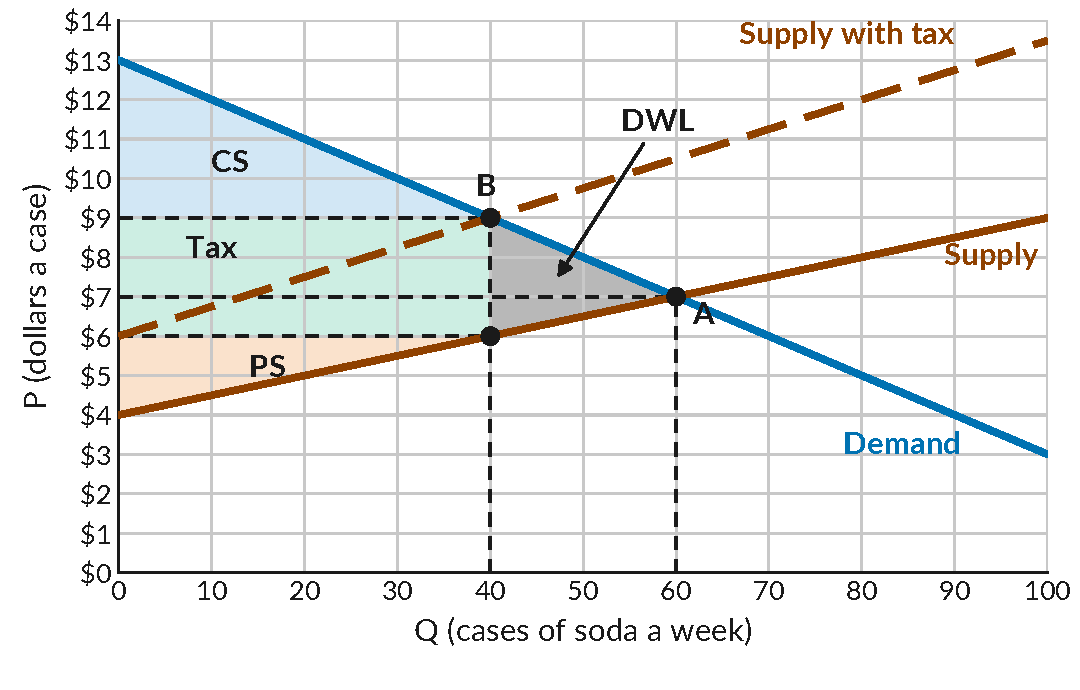
\includegraphics[width=0.74\linewidth, alt={Dollars from 0 to 14 on the vertical axis with gridlines every dollar, and cases of soda a week from 0 to 100 on the horizontal with gridlines every 10. Demand falls from 13 dollars at zero cases to 3 dollars at 100. Supply rises from 4 dollars at zero cases to 9 dollars at 100, and a dashed line labelled Supply with tax rises from 6 dollars, 50 percent above it. A marks 60 cases at 7 dollars. B marks 40 cases at 9 dollars, where demand meets supply with tax, and a dot on the supply curve at 40 cases marks 6 dollars. The triangle between demand and the 9 dollar line is shaded blue, labelled CS. The rectangle between 6 and 9 dollars out to 40 cases is shaded green, labelled Tax. The triangle between 6 dollars and supply out to 40 cases is shaded orange, labelled PS. The triangle from 40 to 60 cases between the curves is shaded grey, labelled DWL.}]{figures/soda-key.pdf}
\else
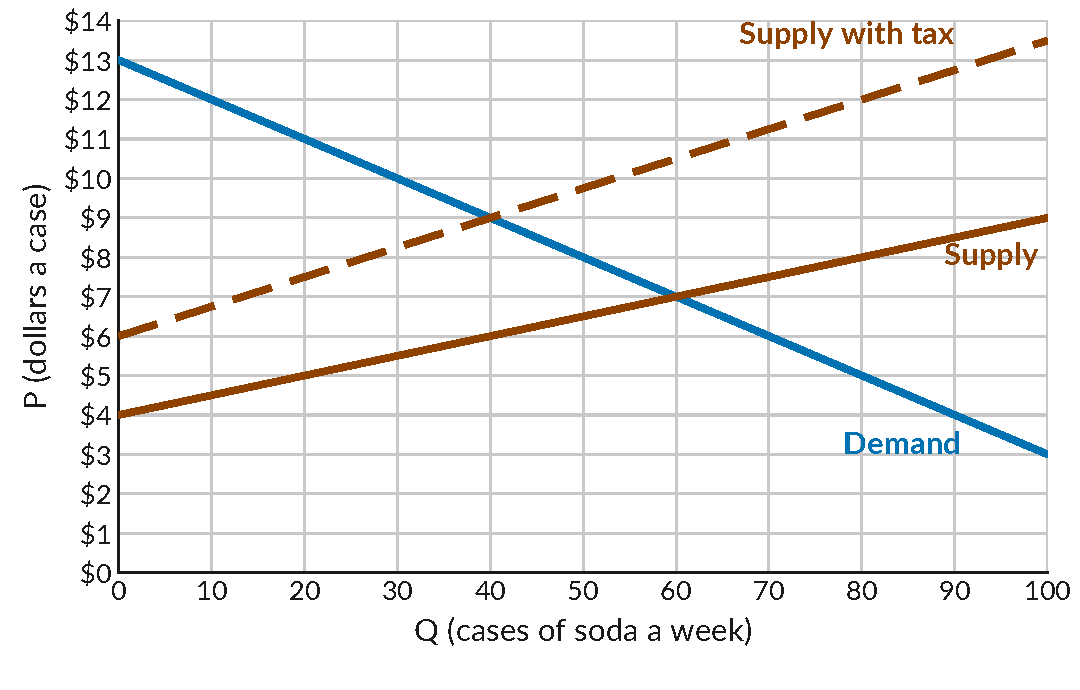
\includegraphics[width=0.74\linewidth, alt={A plotting grid, dollars from 0 to 14 on the vertical axis with gridlines every dollar, and cases of soda a week from 0 to 100 on the horizontal with gridlines every 10. Demand falls in a straight line from 13 dollars at zero cases to 3 dollars at 100. Supply rises in a straight line from 4 dollars at zero cases to 9 dollars at 100. A dashed line labelled Supply with tax rises from 6 dollars at zero cases, passing through 9 dollars at 40 cases.}]{figures/soda.pdf}
\fi
\end{center}

\qpart{a}{1} What are the equilibrium price and quantity before the tax? Mark this point, $A$, on the graph.
\work{1.5}
\sol{\$7 and 60 cases, where demand crosses supply. At that price buyers want exactly what sellers want to sell.}

\qpart{b}{1.5} With the tax, how many cases are sold, what price do buyers pay, and what price do sellers keep? Mark the point where buyers trade, $B$, on the graph.
\work{2}
\sol{40 cases, where demand crosses supply with the tax. Buyers pay \$9, the height of demand at 40 cases. Sellers keep \$6, the height of the original supply curve at 40 cases, since that is what they need to keep to be willing to sell 40. The \$3 between them goes to the city, and it is 50\% of \$6.}

\qpart{c}{1.5} On the graph, shade and label the consumer surplus, the producer surplus, the tax revenue, and the deadweight loss with the tax.
\sol{See the plot above. Consumer surplus is what buyers would have paid above \$9. Tax revenue is \$3 on each of the 40 cases. Producer surplus is what sellers keep above their costs. The deadweight loss is the triangle over the cases from 40 to 60, which are no longer sold.}

\ifsolutions\else\clearpage\fi
\qpart{d}{1} Calculate the consumer surplus and the producer surplus with the tax, using the area of a triangle, $\tfrac{1}{2} \times \text{base} \times \text{height}$. Do buyers or sellers get the larger share?
\ifsolutions\else\vspace{\stretch{2}}\fi
\sol{$\text{CS} = \tfrac{1}{2} \times 40 \times (13 - 9) = 80$ and $\text{PS} = \tfrac{1}{2} \times 40 \times (6 - 4) = 40$. Buyers get the larger share: demand is steep, so many buyers value soda well above what they pay.}

\qpart{e}{1.5} The law says sellers pay this tax. How much of the \$3 tax do buyers bear, and how much do sellers bear? Calculate each side's share of the tax as a percentage.
\ifsolutions\else\vspace{\stretch{3}}\fi
\sol{Buyers pay $9 - 7 = 2$ more than before, and sellers keep $7 - 6 = 1$ less. So buyers bear $2 / 3 = 67\%$ of the tax and sellers $1 / 3 = 33\%$, even though sellers are the ones who hand the money to the city.}

\qpart{f}{1.5} Explain why buyers bear more of the tax here.
\ifsolutions\else\vspace{\stretch{3}}\fi
\sol{Buyers do not cut back much when soda gets more expensive, so sellers can pass most of the tax on to them. Sellers cut back more readily when what they keep falls, so the price they keep does not have to fall as far.}

\qpart{g}{1} Suppose many close substitutes for soda appeared, so demand became much flatter. How would the split of the tax change, and would the quantity sold fall by more or by less?
\ifsolutions\else\vspace{\stretch{3}}\fi
\sol{With close substitutes, buyers switch away when the price rises, so sellers cannot pass on as much of the tax: sellers bear more and buyers less. And since buyers walk away more easily, the quantity sold falls by more.}

\qpart{h}{1} What does the deadweight loss represent here?
\ifsolutions\else\vspace{\stretch{3}}\fi
\sol{The 20 cases no longer sold, from 40 to 60. Each was worth more to a buyer than it cost to supply, so those sales would have left both sides better off. The tax stops them, and nobody gets that surplus: not buyers, not sellers, not the city.}
